\documentclass[11pt]{article}
\pdfinfoomitdate=1\pdftrailerid{}
\usepackage[letterpaper,margin=.7in,headheight=15pt,headsep=18pt,footskip=24pt]{geometry}
\usepackage[T1]{fontenc}
\usepackage{lmodern,amsmath,amssymb,array,booktabs,fancyhdr,tikz,hyperref}
\renewcommand{\familydefault}{\sfdefault}
\setlength{\parindent}{0pt}\setlength{\parskip}{6pt}
\pagestyle{fancy}\fancyhf{}
\fancyhead[L]{\small Week 58 / Fair division / Adult return-visit guide}
\fancyfoot[L]{\scriptsize Bellingham Math Circle / Week 58 / W58-RV-FAC-v1}
\fancyfoot[R]{\thepage}
\newcommand{\head}[1]{\par\textbf{\large #1}\par}
\newcommand{\sub}[1]{\par\textbf{#1}\par}
\newcommand{\hint}[1]{\textit{If needed:} #1}
\newcommand{\seq}[1]{\texttt{#1}}
\hypersetup{hidelinks}
% Generated and rechecked by check_guide.py; do not edit by hand.
\newcommand{\ktable}{%
\begin{tabular}{@{}rll@{}}
\textbf{Row} & \textbf{Train with minimum cuts} & \textbf{Fewest}\\\midrule
1 & \texttt{RB|RB} & 1\\
2 & \texttt{R|RB|B} & 2\\
3 & \texttt{BR|RB} & 1\\
4 & \texttt{B|BR|R} & 2\\
5 & \texttt{RB|BR} & 1\\
6 & \texttt{BR|BR} & 1\\
\end{tabular}}
\newcommand{\ksecond}{%
\begin{tabular}{@{}rll@{}}
\textbf{Row} & \textbf{Train with minimum cuts} & \textbf{Fewest}\\\midrule
1 & \texttt{RR|RRB|B} & 2\\
2 & \texttt{BRR|BRR} & 1\\
3 & \texttt{RBRBR} & impossible\\
4 & \texttt{RRBB|BBRR} & 1\\
5 & \texttt{RR|RRBB|BB} & 2\\
6 & \texttt{RRRBB|BBRRR} & 1\\
7 & \texttt{RRR|RRRBB|BB} & 2\\
\end{tabular}}
\newcommand{\msecond}{%
\begin{tabular}{@{}rll@{}}
\textbf{Row} & \textbf{Train with minimum cuts} & \textbf{Fewest}\\\midrule
1 & \texttt{RR|RRB|B} & 2\\
2 & \texttt{RB|BRR|R} & 2\\
3 & \texttt{BRRB|RRBB} & 1\\
4 & \texttt{R|RRBB|BBR} & 2\\
5 & \texttt{RBRRBRB} & impossible\\
6 & \texttt{RR|BRRRB|BBR} & 2\\
7 & \texttt{RBBRR|RRBBR} & 1\\
\end{tabular}}
\newcommand{\utable}{%
\begin{tabular}{@{}rll@{}}
\textbf{Row} & \textbf{Train with minimum cuts} & \textbf{Fewest}\\\midrule
1 & \texttt{R|RRBB|BBR} & 2\\
2 & \texttt{BRRB|RBBR} & 1\\
3 & \texttt{RR|RRBB|BB} & 2\\
4 & \texttt{RBRR|RRBRB|B} & 2\\
5 & \texttt{BBRRR|RRRBB} & 1\\
6 & \texttt{RRR|RRRB|B} & 2\\
\end{tabular}}
\newcommand{\allfour}{%
\begin{tabular}{@{}lll@{}}
\textbf{Train} & \textbf{Cuts} & \textbf{Fewest}\\\midrule
\texttt{BBRR} & \texttt{B|BR|R} & 2\\
\texttt{BRBR} & \texttt{BR|BR} & 1\\
\texttt{BRRB} & \texttt{BR|RB} & 1\\
\texttt{RBBR} & \texttt{RB|BR} & 1\\
\texttt{RBRB} & \texttt{RB|RB} & 1\\
\texttt{RRBB} & \texttt{R|RB|B} & 2\\
\end{tabular}}
\newcommand{\gametable}{%
\begin{tabular}{@{}lllll@{}}
\textbf{Order} & \textbf{First marks A B C} & \textbf{First taker} & \textbf{Second marks} & \textbf{Second taker}\\\midrule
X Y Z & 50, 100, 25 & C at 25 & A: 62.5, B: 100 & A at 62.5\\
X Z Y & 50, 75, 25 & C at 25 & A: 112.5, B: 75 & B at 75\\
Y X Z & 25, 50, 75 & A at 25 & B: 112.5, C: 75 & C at 75\\
Y Z X & 25, 50, 100 & A at 25 & B: 62.5, C: 100 & B at 62.5\\
Z X Y & 100, 25, 50 & B at 25 & A: 100, C: 62.5 & C at 62.5\\
Z Y X & 75, 25, 50 & B at 25 & A: 75, C: 112.5 & A at 75\\
\end{tabular}}
\newcommand{\scoretable}{%
\begin{tabular}{@{}lllll@{}}
\textbf{Order} & \textbf{A sees A B C} & \textbf{B sees A B C} & \textbf{C sees A B C} & \textbf{Envy}\\\midrule
X Y Z & 4, 6, 2 & 1, 11, 0 & 4, 4, 4 & A to B\\
X Z Y & 8, 2, 2 & 8, 4, 0 & 2, 6, 4 & B to A, C to B\\
Y X Z & 4, 2, 6 & 2, 8, 2 & 0, 8, 4 & A to C, C to B\\
Y Z X & 4, 4, 4 & 2, 4, 6 & 0, 1, 11 & B to C\\
Z X Y & 11, 0, 1 & 4, 4, 4 & 6, 2, 4 & C to A\\
Z Y X & 4, 0, 8 & 6, 4, 2 & 2, 2, 8 & A to C, B to A\\
\end{tabular}}

\begin{document}
\head{Mathematical overview}
\textbf{Two colours need at most two cuts.} A nonempty row with an even number of reds and an even number of blues can be shared into two trays with half of each colour using at most two gaps. Cards stay whole; the order within each piece stays fixed; a tray may receive several pieces. An odd count of either colour makes equal sharing impossible, not a three-cut example.

\textbf{Proof by a moving window.} Write the counts as $2r$ reds and $2b$ blues. A window of $r+b$ consecutive cards starts at the left end and moves one card at a time to the right end. If its first red count is $q$, its last red count is $2r-q$, because those end windows partition the train. Each step changes that count by at most one. It must therefore reach $r$. That window also has $b$ blues. Give the window to one tray and the outside pieces to the other. At an end this uses one gap; inside it uses two. One cut is possible exactly when the first half already has half of each colour.

\textbf{Exact halves are stronger than a fair choice.} On the two-colour strip, half of each colour gives half the value to \emph{every} taste that is additive and uniform within each colour. This holds for any nonnegative values on the two-person cards, including zero. For the printed opposite tastes, the equal-value equations force half of each colour; one straight-across cut cannot do that. Three independent tastes can need three cuts: on X, Y, Z the printed cards force half of \emph{each} panel. The algebra and attaining cuts appear with the solutions. These are complete allocations: nothing is discarded.

\textbf{The marking game guarantees a third, not freedom from envy.} Let person $i$ value the whole row at $T_i$, with fixed, nonnegative additive values and continuous accumulation along the row. At each round each remaining person marks a prefix of value $T_i/3$, measured from the new left end. The leftmost marker takes that prefix. A taker receives exactly their third; every removed prefix was worth at most $T_i/3$ to anyone still waiting. Thus the last person keeps at least $T_i-2T_i/3=T_i/3$. Enough value remains for the next mark. Tied leftmost marks may be resolved either way. A zero-total person can take the empty prefix; the bound is still valid. In these panels $T_i=12$, so the target is always 4, \emph{not a third of the remainder}.

\textbf{Only two cards can be split.} There are two selected cut locations in a three-person marking game on a row of cards. Each cuts at most one card; a gap cuts none. Other pencil marks are not cuts. This bound can be necessary. The general $n$-person version targets $T_i/n$ and uses at most $n-1$ cut locations, under the same divisible-value assumptions.

\textbf{Discovery and band map.} The first visit used cut-and-choose and compared each tray with one fixed observer's card. Here children seek exact equality for both observers, minimize cuts, and separate a guaranteed share from a desirable outcome. K--1 matches colours and counts to six, with adult reading. Grades 2--3 organizes colour orders, uses halves and small sums, and may try three-person roles. Grades 4--5 explains the moving window, uses fractions and three observers, and proves guarantees. Experiments suggest a rule; a full small catalogue or an argument establishes it. Physical cuts only approximate exact lengths.
\newpage
\head{Preparation and a manageable hour}
\textbf{Status.} Unpiloted and physically unrehearsed. Print scale, tray fit, handling ten-card trains, cutting at marked points, quarter-panel marks, staffing and timings have not been tested with this return visit.

\textbf{Reuse W58-materials-v3.} Print \texttt{week-58-materials.pdf} single-sided on US Letter at Actual Size, with pages 2--8 landscape. Check the 100 mm bars. Cut outside borders; no page is a working mat. Build on the table and record on the student pages. Student strip pictures are schematic, not ruler-sized cutting stock.

\begin{tabular}{@{}p{.12\linewidth}p{.82\linewidth}@{}}
\textbf{Page} & \textbf{Contents and use}\\\midrule
1 & Five 25 mm squares R1, R2, R3, B1, B2, plus a separate paper R3. Keep the base five sturdy; leave disposable copies unmounted.\\
2 & Two-person A/B cards, each $100\times150$ mm; numbers value a whole 120 mm colour panel on a strip.\\
3 & U/V cards, each $100\times150$ mm; every red is worth 1. Upper student Problem 8 also specifies blue value 0.\\
4--5 & Three-person A/B/C cards, each $100\times150$ mm. Page 5 also has X/Y/Z panels, each $50\times40$ mm.\\
6--8 & Three $240\times40$ mm red/blue strips per page, nine per full pair stock. Red and blue are each 120 mm long.\\
\end{tabular}

\textbf{Per pair.} One base goods kit plus one extra unmounted page 1 supplies six reds and four blues for the longest fixed trains. Set the extra paper R3 aside; do not add it as a seventh red. Supply two 150--180 mm trays, one ruler, pencils, red/blue crayons (or draw circles/squares), and scrap paper. Reserve a 300 mm clear table run for ten touching cards. For strips use two flat zones at least $180\times100$ mm, with room for the initial 240 mm strip. Start with three fresh strips per pair (page 6); refill from pages 7--8 when needed. No scissors are used on train cards.

\textbf{Per table.} Two pairs at K--1 and 2--3 need 12 reds, 8 blues and four trays in total; the upper pair needs six reds, four blues and two trays. For each active three-person game use three trays and one complete three-person A/B/C set. The fourth middle-table child referees; at the upper trio the adult referees. Put the two-person A/B cards away before the panel game: the letters repeat but their values differ.

\textbf{Consumables for all later tasks.} Budget four fresh page-5 panel sets at the middle table (three games and a spare), eight at the upper table (one exact-half trial, six games and a spare). These are totals, including any unused base sets; print extra page 5 as needed. Print page 4 once for each table lacking the three-person A/B cards. Keep the upper paper R3 for Problem 7; one further unmounted page 1 supplies two fresh paper reds for Problem 8. For five simultaneous pairs, the train addition is five page-1 copies. Adults hold the three scissors, cut only after checking children's marks, and keep panel fragments labelled.

\textbf{Time and staffing.} With the base kit ready, allow 20--30 minutes to print, cut and bag additions; this is an estimate. Anchor one adult at each band: read or scribe, maintain the correct observer and supervise cuts, but let children choose arrangements and marks. Use 5 minutes of movement, 5 for handling/launch, 35 for investigations, 5 for a stretch/reset and 10 for sharing. K--1: Problems 1--2, then 3 if wanted; save 4--5. Middle: Problems 1--3; save 4--6 or choose the panel game instead of strips. Upper: Problems 1--3 and perhaps 4; give Problems 5--8 another visit. Keeping one investigation going is better than finishing every page.
\newpage
\head{Shared launch and K--1 solutions}
\textbf{Launch together, about five minutes.} Let children handle cards and trays first. Reuse the opening non-task example, \seq{RBRBRR}. Point to the chosen gap, move both intact pieces into trays, and compare colour counts, not the order within a tray. Say that a tray may hold several pieces, but do not demonstrate the two-cut trick. Count marked gaps, not hand motions. All three packets print this example before Problem 1.
\begin{center}
\begin{tabular}{ccc}
Input & Mark one gap & Output\\[3pt]
\seq{RBRBRR} & \seq{RBR|BRR} & tray 1: \seq{RBR}\quad tray 2: \seq{BRR}
\end{tabular}
\end{center}
Before any strip or panel task, show a straight-across cut on scrap. For a new length/value convention use this separate neutral example, not a task panel:
\begin{center}
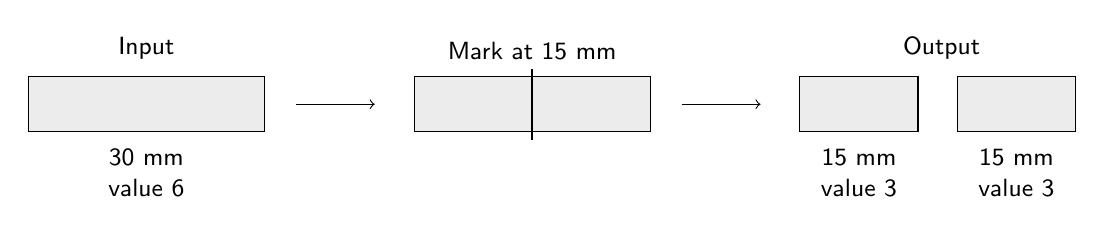
\begin{tikzpicture}[x=1mm,y=1mm,font=\small]
\draw[fill=gray!15] (0,0) rectangle (30,7);
\node[above] at (15,8) {Input};\node[below,align=center] at (15,-1) {30 mm\\value 6};
\draw[->] (34,3.5)--(44,3.5);
\draw[fill=gray!15] (49,0) rectangle (79,7);\draw[thick] (64,-1)--(64,8);
\node[above] at (64,8) {Mark at 15 mm};
\draw[->] (83,3.5)--(93,3.5);
\draw[fill=gray!15] (98,0) rectangle (113,7);\draw[fill=gray!15] (118,0) rectangle (133,7);
\node[above] at (116,8) {Output};
\node[below,align=center] at (105.5,-1) {15 mm\\value 3};
\node[below,align=center] at (125.5,-1) {15 mm\\value 3};
\end{tikzpicture}
\end{center}
This paper can be made from scrap; the base kit does not print it. Later, read the panel-game's printed first-round example at its table before children play. Do not launch all three investigations at once.

\textbf{Adult key notation.} R is a red circle card, B a blue square card; a vertical bar is a cut \emph{between} cards. With two bars give the middle piece to one tray and the two ends to the other. Row numbers below count down the page and are not additional problem numbers.

\begin{minipage}[t]{.46\linewidth}
\sub{Problem 1 on student page 1}
\small\ktable
\end{minipage}\hfill
\begin{minipage}[t]{.50\linewidth}
\sub{Problem 2 on student page 2}
\small\ksecond
\end{minipage}

\textbf{Problem 1 reasoning.} Each tray needs one red and one blue. A single cut must be at the middle; in rows 2 and 4 that gives one tray only reds and the other only blues. The displayed two-cut divisions work, so two is minimal. These are the only minimum gap positions, apart from swapping trays. \hint{``What must each tray have? Does changing the order in a tray change its counts?''}

\textbf{Problem 2 reasoning.} Row 3 has three reds, which cannot be matched across two trays. For every other row, a one-gap share must leave half the cards on each side. Testing that single middle gap proves the displayed minimum. The two end pieces may sit separately in the same tray. \hint{``Can you pair every red with one in the other tray? Could one tray hold two pieces?''}
\newpage
\head{K--1 continuations and middle train work}
\sub{K--1 Problem 3 on student page 3}
A successful challenge has four reds and four blues, but its first four cards do \emph{not} contain two reds. One gap would have to split eight cards into four and four, so there is no other one-gap position to try. There are 34 such colour orders out of 70; the other 36 have two reds among their first four. For completeness, the failing first-half red counts are 0, 1, 3, 4, giving $1,16,16,1$ orders respectively. Within each class, choose the red positions in each half; this describes every answer without a 34-row catalogue.

The revised prompt is a partner game: record each successful challenge actually played, not all 34. Seven blank rows are not a promised answer count. \seq{RRRRBBBB} is one example; do not supply it before children invent their own. \hint{``If both trays need four cards, which gap could possibly work?''} A later continuation is to share the same challenge with two gaps rather than invent more one-gap failures.

\sub{K--1 Problem 4 on student page 4}
Use the separate $240\times40$ mm strip. Two cuts at \textbf{60 and 180 mm from the red end} work: the middle piece and the two ends each contain 60 mm red and 60 mm blue. One straight-across cut cannot split both colours. These are the unique minimum cut positions. Children can fold or match colour lengths; an adult measures and cuts where the child marks. \hint{``Does each tray have half of \emph{each} colour? Which colours would one cut split?''} Do not accept a lengthwise cut: the printed rule now says straight across.

\sub{K--1 Problem 5 on student page 5}
\textbf{No shareable train needs three gaps.} Even counts always permit at most two by the overview's window argument. Odd-count trains are impossible and do not answer the question. Within the six-red/four-blue supply, exhaustive checking of all 790 nonempty colour trains gives 441 impossible, 179 one-gap and 170 two-gap trains. These are adult checks, not a K--1 enumeration assignment. \hint{``Can this train be shared at all? Can a middle piece match the two ends?''} Let a child demonstrate several hard trains; save the general proof for a ready group.

\sub{Grades 2--3 Problem 1 on student page 1}
These are all six colour orders; swapping labels on same-colour cards does not create a new one. Reversing a colour order does count as a different row when the word changes.
\begin{center}\allfour\end{center}
Completeness: choose the two red places among four, giving $\binom42=6$. Alternatively group by the first red's position: first place gives three choices for the other red, second gives two, third gives one. Eight recording rows include spare space. \hint{``How could you sort your trains so that you notice a missing one?''} Children can pool records rather than each reproduce a catalogue.
\newpage
\head{Grades 2--3 solutions and the marking game}
\sub{Problem 2 on student page 2}
\begin{center}\msecond\end{center}
Row 5 has three blues and is impossible. For every other row, test the unique middle gap to rule out one cut; the table gives an attaining division. Row 6 has exactly two minimum choices: gaps after cards $(2,7)$ or $(3,8)$, namely \seq{RR|BRRRB|BBR} and \seq{RRB|RRRBB|BR}. All other displayed shareable rows have one minimum choice. \hint{``If one cut worked, how many cards would be on each side?''}

\sub{Problem 3 on student page 3}
The answer is the same 60/180 mm division as K--1 Problem 4. Both people give the middle piece value $3/2+1/2=2$, and the ends together value 2. A single cut exact for A is at 80 mm; B's is at 160 mm, so no single cut is exact for both. Read real lengths from the material strip, not a ruler laid on the schematic student picture. \hint{``Use A's card on both trays, then B's on both. What does half a colour contribute?''} The upper Problem 3 solution supplies uniqueness and arbitrary-value reasoning.

\sub{Problem 4 on student page 4}
\textbf{No.} The even-count hypothesis gives the two-gap window proof on guide page 1. If children conjecture the bound after experiments, ask, ``Could a block holding half the cards have too many reds at both ends of its trip?'' Use fingers or scrap paper as a movable window only after a need for an explanation arises. The printed twelve-card records are capacity, not a required length: the ten-card kit is enough to investigate; sketch any larger invented train. One counterexample would disprove an ``always'' claim, but many failed searches do not prove it.

\sub{Problems 5 and 6 on student pages 5 and 6}
Use three-person A/B/C and three trays. Page 5's worked XYZ first round is a rule example; the first task game is \textbf{XZY}. Problem 6 adds \textbf{YXZ and ZYX}. For those three games the actual cuts are at 25 and 75 mm. The first and second takers each get own value 4; the remaining person gets 8. Nobody gets less than 4, but somebody envies in each game. The full lookup table on guide page 7 also serves upper Problem 5.

\textbf{Quarter marks still arise.} In each middle game one second-round non-taker marks at 112.5 mm: 12.5 mm into the last panel. A quarter of a panel worth 8 is worth 2. The half-panel demonstration on student page 5 does not teach this quarter; let the adult scribe that mark if needed. Children can establish that this person's mark lies past 75 mm without measuring it exactly, but do not pretend that it is a half-panel point.

\hint{``From the \emph{new} left end, what does your own card value? Now keep that same card and check all three trays.''} If the adult must choose the marks rather than read or record them, pause the game and return to one-panel halves. As a later challenge, ask whether a fair third can coexist with wanting another tray; do not compare different people's own scores as an envy test.
\newpage
\head{Upper exact halves and fewest cuts}
\sub{Problem 1 on student page 1}
\begin{center}\utable\end{center}
All displayed trains are shareable, and each has a unique minimum set of gap positions. In row 4 the middle window is cards 5--9; it need not be centred in the whole train. For four reds and four blues, one cut works exactly when the first four cards have two reds and two blues: there are $\binom42\binom42=36$ such orders among $\binom84=70$. The other 34 need two cuts. \hint{``Where would the only possible one-cut division be?''}

\sub{Problem 2 on student page 2}
\textbf{No even-count two-colour train needs more than two cuts.} Use the overview's moving-window proof. Children may act the proof by shifting a half-length window one card and explaining that at most one red is lost and at most one enters. The first and last windows are complements, so a red surplus must become a deficit unless a balanced window has already appeared. \hint{``Can a whole-number count jump from too many to too few without passing the target?''} More colours are a different problem, not a counterexample to this theorem.

\sub{Problem 3 on student page 2}
\textbf{Exactly two cuts, uniquely at 60 and 180 mm}, up to exchanging trays. If a tray holds fractions $r$ of the red and $b$ of the blue, being exact for both people means
\[
3r+b=2,\qquad r+3b=2.
\]
Subtract to get $r=b$, then $r=b=1/2$. With two genuine cuts and two trays, the middle piece must be in one tray and both end pieces in the other; otherwise a cut could be removed. The middle must contain 60 mm of each colour, forcing the two positions. One cut cannot split both colours; alternatively A's unique one-cut half is 80 mm and B's is 160 mm.

\textbf{Any other numbers on these two-colour cards still work with the same cuts.} Half of each colour contributes $(a+b)/2$ for a card valuing the whole panels at $a,b$. This includes zero-valued panels and identical tastes, where one cut may suffice and minimum answers need not be unique. No advanced theorem is needed for this question on these two uniform panels. \hint{``Which fraction of each colour would work regardless of its price?''} Changing the density \emph{within} colours is a different generalization.

\sub{Problem 4 on student page 3}
\textbf{Three cuts are necessary and sufficient.} Cut each of X, Y, Z in half: at 25, 75 and 125 mm along the row. Give each tray one half of every panel, so each is worth 6 to all three observers. To see why fewer cannot work, let $x,y,z$ be the fractions in one tray. The conditions are
\[
x+2y=3/2,\qquad y+2z=3/2,\qquad 2x+z=3/2.
\]
Their sum gives $x+y+z=3/2$. Comparing with the first equation gives $y=z$; comparing with the second gives $z=x$. Thus all are $1/2$. Each panel needs an interior cut, so at least three are needed. The $3\times3$ value matrix has determinant 576, another check of uniqueness of these fractions. \hint{``Could a whole panel go to just one tray if each observer still saw a tie?''} This proves the panel fractions and cut positions, not that only one physical arrangement of halves in trays is allowed.
\newpage
\head{All marking games and the upper guarantee}
\sub{Grades 4--5 Problem 5 on student page 4}
Finish XYZ, then try the other five orders. Every coordinate below is in millimetres from the \emph{original} left end of the $150$ mm row. First cut at the first taker's mark; second cut at the second taker's mark; the last person receives everything after it. For example, XYZ gives C $[0,25]$, A $[25,62.5]$, B $[62.5,150]$. Brackets here describe lengths; shared endpoints carry no value.
\begin{center}\small\setlength{\tabcolsep}{4pt}\gametable\end{center}
All six orders are listed, since three distinct panels have $3!=6$ orders. No selected marks tie. XYZ, YZX and ZXY need a quarter-panel cut; the others cut at half-panel points. Allow children to distribute the six trials across pairs or visits and pool records.

\textbf{Complete observer check.} In each triple below the entries value \emph{A's, B's, C's trays in that order}, using only the named observer's card. ``A to B'' means A strictly prefers B's tray. Equal values do not count as envy.
\begin{center}\small\setlength{\tabcolsep}{5pt}\scoretable\end{center}
Thus nobody gets less than 4. The last person's own value is 11 in XYZ, YZX and ZXY, and 8 in XZY, YXZ and ZYX. The two takers have exactly 4. The envy column is complete, not just one example per game. \hint{``Which row of numbers uses your card throughout? Is your own tray at least as valuable as each other one?''}

\sub{Grades 4--5 Problem 6 on student page 5}
The proof is the marking invariant on guide page 1. A child can explain it with three spaces labelled ``taken'', ``taken'', ``left'': each taken space was worth at most 4 to the person left waiting, leaving at least $12-4-4=4$. A taker gets exactly 4 by their own mark. Each still-waiting person retains enough value to make the next mark, so the procedure does not get stuck.

\textbf{The printed generalization needs a qualification.} ``Whatever values the cards give'' is valid when each person aims at one third of \emph{their own original total}, not the fixed number 4 unless that total remains 12. If all three panels were worth 8 to everyone, total 24, taking value 4 would fall below the required 8. For changed cards, announce the new personal targets before playing. Values must remain nonnegative, additive and uniformly divisible within panels; negative values or indivisible positive-value cards invalidate this argument.

For the printed cards, giving A whole Y, B whole Z and C whole X gives everyone 8 and no envy: each sees the other two whole panels as 4 and 0. \textbf{The marking game cannot do that well for all three}, in any order: its first two takers receive exactly 4. A guarantee is a floor, not the best allocation. \hint{``What value does the rule force the first taker to receive? What might that person think of a larger tray left later?''}
\newpage
\head{Upper card continuations and sources}
\sub{Problem 7 on student page 5}
By two-person card A, three reds and two blues total $3+1+3+1+3=11$. Half is $5.5$. In the printed R1 B1 R3 B2 R2 row, cut halfway through paper R3, \textbf{62.5 mm from the left} of the 125 mm row. Each side has one red, one blue and half a red: $3+1+1.5=5.5$. The red circle names the card; value follows the whole square, not the ink.

\textbf{Neither a gap nor the inside of a blue card can be the half point in any order.} Every whole-card running total is an integer, never 5.5. For a blue of value 1 to straddle 5.5, the preceding cards would have to total 5. The only possibility from these values is one red plus both blues; then no blue remains for the cut. All 120 labelled orders (ten colour orders) agree. \hint{``What totals can you have just before a blue?''} In rearranged trials mark the answer; use an unmounted replacement of whichever red would be cut, never a sturdy card.

\sub{Problem 8 on student page 6}
The marking game makes only two \emph{selected} cuts. A cut at a gap splits no card and a cut inside a card splits just that card. This proves at most two distinct cards are split, even if both cuts happened to lie in the same card. Use the same uniform-within-card rule as Problem 7, and target each person's own third.

\textbf{No, cutting only one of the two paper reds cannot suffice.} The total is 2 and each person needs $2/3$. The uncut red must go whole to someone; the other two would need $4/3$ from the remaining red of value 1. Cutting that one card repeatedly does not help. The bound is attained by cutting the first red at $2/3$ of its width and the second at $1/3$ of its width: the three consecutive shares each have value $2/3$. On two touching 25 mm cards the locations are $50/3$ and $100/3$ mm from the left. \hint{``Who receives the uncut card, and what is left for the other two?''}

\sub{Sources consulted and boundaries}
Consulted for this guide: the final 5/6/6-page return-visit PDFs and their source; the return-visit outline and both earlier reviews; W58-guide-v4, especially pp. 1--3 and 9; W58-materials-v3, pp. 1--8; and the Week 8 return-visit and Week 98 guides as structure models. Earlier answer keys were not treated as final-page authority. The numerical instances and this checker were derived afresh.

Ariel D. Procaccia, \emph{Cake Cutting Algorithms}, author-hosted chapter, \S13.2 (PDF pp. 1--3), \S13.3.1 (p. 4), \S13.3.2 (pp. 4--5), and \S13.3.3 (pp. 5--6), consulted online: \href{https://procaccia.info/wp-content/uploads/2020/03/cakechapter.pdf}{procaccia.info, cakechapter.pdf}. These sections support the value model, cut-and-choose, proportional marking and the distinction from the three-person envy-free procedure. We do not teach Selfridge--Conway here.

\textbf{Outline bibliography, not newly consulted.} A. K. Austin, ``Sharing a cake'', \emph{Mathematical Gazette} 66 (1982), 212--215; C. R. Hobby and J. R. Rice, ``A moment problem in L1 approximation'', \emph{Proc. AMS} 16 (1965), 665--670; C. H. Goldberg and D. B. West, ``Bisection of circle colorings'', \emph{SIAM J. Algebraic Discrete Methods} 6 (1985), 93--106; N. Alon and D. B. West, ``The Borsuk--Ulam theorem and bisection of necklaces'', \emph{Proc. AMS} 98 (1986), 623--628; J. Matou\v{s}ek, \emph{Using the Borsuk--Ulam Theorem} (2003), necklace-splitting treatment (no page locator supplied in the outline). H. Steinhaus, ``The problem of fair division'', \emph{Econometrica} 16 (1948), 101--104; L. E. Dubins and E. H. Spanier, ``How to cut a cake fairly'', \emph{American Mathematical Monthly} 68 (1961), 1--17. Background only: W. Stromquist, same title, \emph{AMM} 87 (1980), 640--644; F. E. Su, ``Rental harmony'', \emph{AMM} 106 (1999), 930--942. General necklace and connected envy-free theorems are not needed or proved here.

\textbf{After use.} Record which problems children chose, where adult reading became adult decision-making, and whether the cutting conventions and observer comparisons were retained. Digital mathematical and page checks do not establish physical readiness or successful classroom use.
\end{document}
